%%%%%%%%%%%%%%%%%%%%%%%%%%%%%%%%%%%%%%%%%%%%
\section{Content Delivery: An Overview}\label{sec:overview}
%%%%%%%%%%%%%%%%%%%%%%%%%%%%%%%%%%%%%%%%%%%%

While content may be seen as king not all content is equally popular among
users. Indeed, content popularity often follows ``Zipf's law''.  If the
popularity of elements as function of the rank is consistent with a power-law
distribution it is referred to as Zipf's-like (see~\cite{Zipf49,Mitzenmacher03}
and references therein).  The rank is determined by the number of occurrence of
an element, where a low rank index refers to a popular element.  Not
surprisingly Zipf's law does not only apply to the popularity of content but
also quite a number of different quantities in Internet traffic, including the
popularity of Web pages~\cite{breslau:99,SerpanosKarakostasWolf:00}, traffic
demands~\cite {Fang_Peterson:1999, feldmann:00,
ZhangBreslauPaxsonShenker2002,Wallerich:2005, BrownleeClaffy02}, as well as
interdomain Web traffic demands~\cite{Feldmann:Kammenhuber:2004}.  Thus, while
some content can be served by a single server most content, namely the popular
content, can only be served if it is highly replicated across multiple servers.
Thus, one of the main challenges in content delivery is {\bf{server
selection}}. Server selection means identifying a specific server from which
the request for content by a user is satisfied.

Content delivery and the network infrastructure interact mostly through content
source selection, often called server selection. Here, it does not matter
whether the source is a server pushing content through HTTP or from a peer in a
P2P network. In the case of HTTP, the domain name system (DNS) is the preferred
mechanism for performing server selection. In the case of P2P, peer selection
strategies drive where the content is obtained from and how, e.g., when the
content is cut into chunks.

To direct users to appropriate servers, CDIs rely extensively on the Domain
Name System (DNS).  We describe this and other server selection mechanisms in
detail later in this section.  The CDI chooses a server based on several
metrics. Criteria for server selection include the IP address of the end-user's
DNS resolver, the availability of the server, the proximity of the server to
the resolver, and the monetary cost of delivering the content. Note that the
server selection does not know the client IP address or network location, it
only knows the IP address of the DNS resolver the end-user contacted. A recent
study~\cite {DNS-IMC-2010} showed that sometimes the end-user is not close to
the resolver. To improve the mapping of end-users to servers, the client-IP
eDNS extension~\cite {DNS-extension-IP-client} has been recently proposed.

In P2P systems peers can choose among all other peers to download content from
but only if the have the desired content. Thus the problem of getting content
in a P2P system is actually two-fold: first the user needs to find the content
and once it knows of possible peers it can download the content from, it needs
to connect to some of them to get the desired content.  In P2P systems the
content lookup is realized in many different ways. Some P2P network, called
structured P2P, implement a distributed lookup system most often referred to as
distributed hash table (DHT). Other P2P systems, called unstructured P2P, like
Gnutella, flood search request into the network.  Some systems rely on a
partial centralized infrastructure to obtain content information. We discuss
the different approaches in P2P systems in more detail in
section~\ref{sec:P2P}.

Before we can discuss all the various options on how content delivery can be
improved in the current Internet we give a short overview how a typical Content
Distribution Network operates.


\subsection{Content Delivery Networks} \label{sec:content_delivery}

\begin{figure} \begin{center}
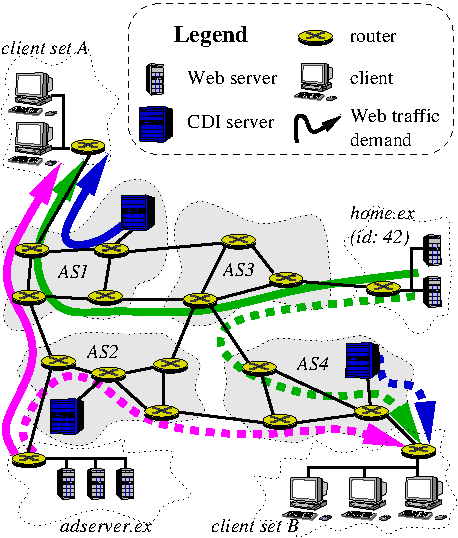
\includegraphics[width=0.7\linewidth]{figures-pdf/flows-example} 
\end{center}
\caption{Example of CDI deployment and traffic flows (Web traffic demands).}
\label{fig:aka:cdn} \end{figure}

\begin{figure} 
\begin{center}
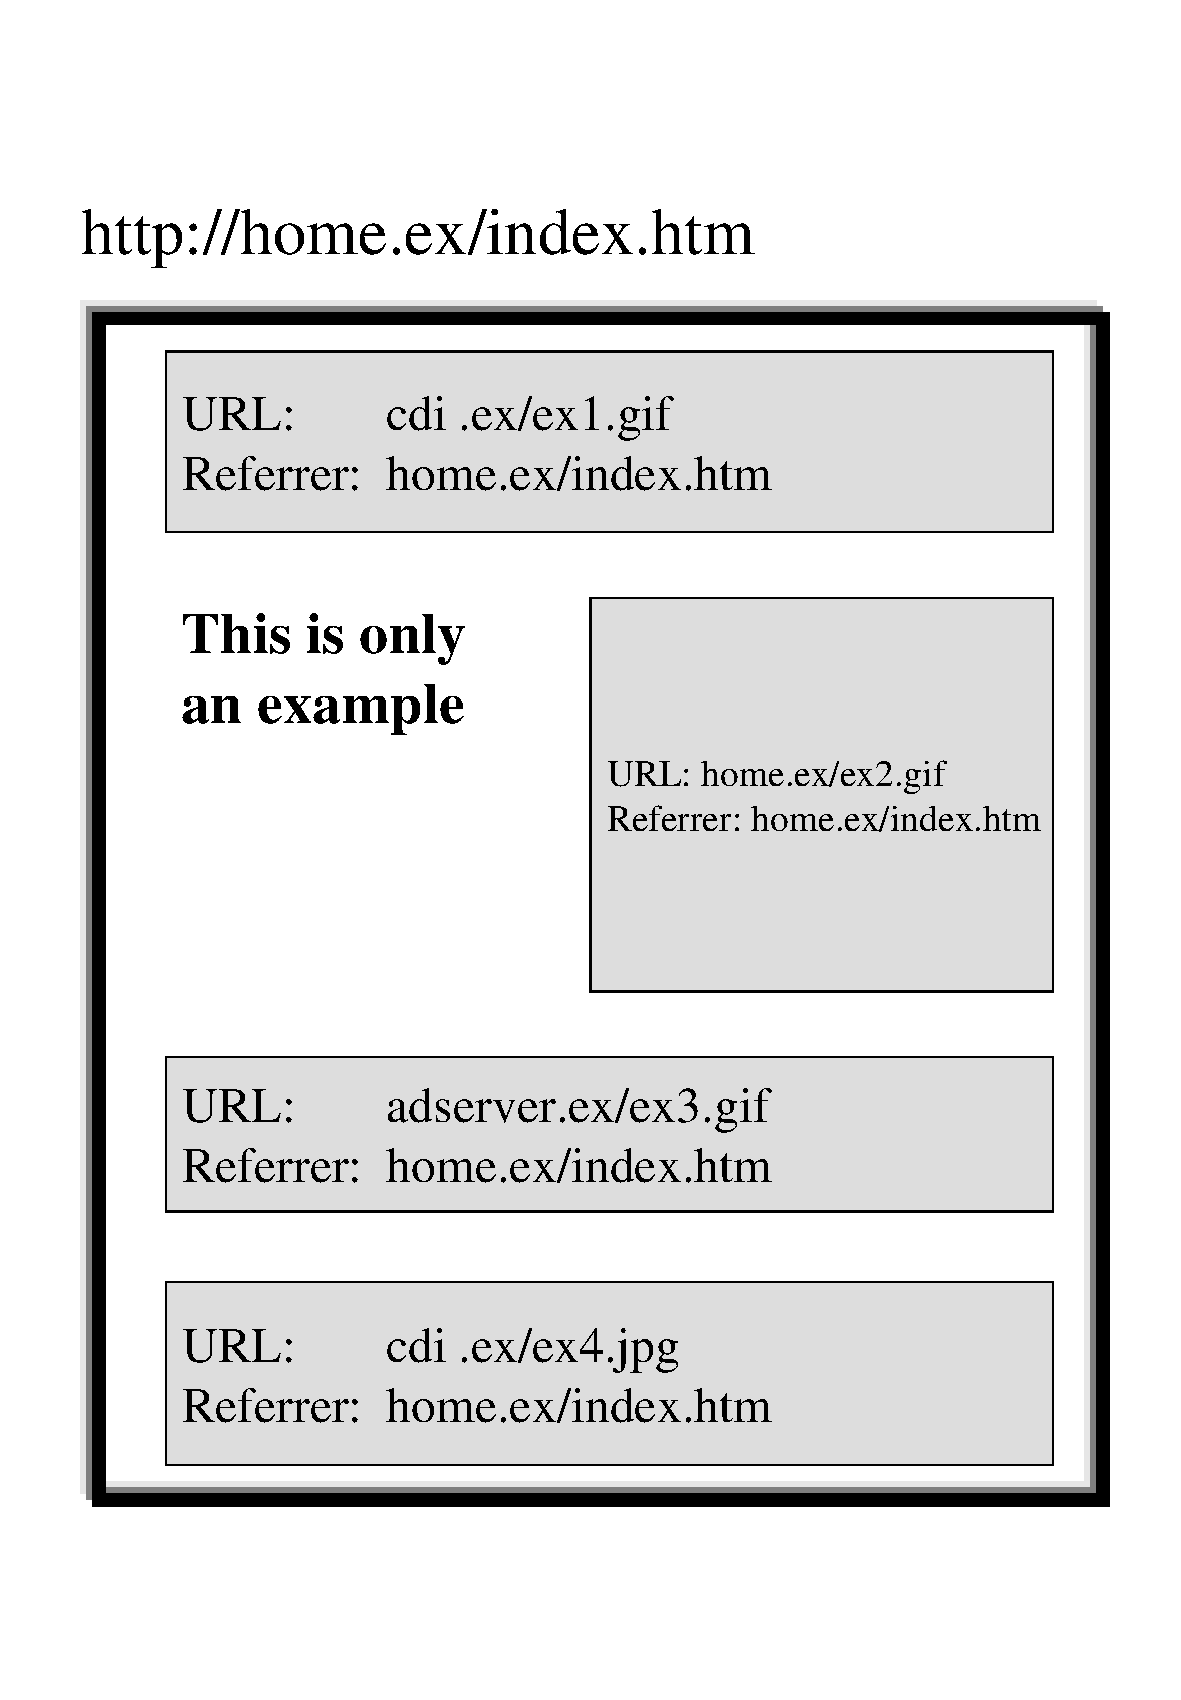
\includegraphics[width=0.6\linewidth]{figures-pdf/page}
\vspace*{-.7cm}
\end{center}
\caption{Example Web page with some CDI content.}
\label{fig:aka:cdn_page}
\end{figure}

Recall content is king in the current Internet and content is typically first
placed on the Web site of the content producer, the original Web servers.
Content Delivery Infrastructures (CDIs) (see,
\eg~\cite{cdn:2002,akamai:2002,gadde01web,bent02whole,johnson00measured,bala:imw01,gribble:osdi02})
are designed to reduce the load on origin servers and at the same time improve
performance for the user.  Most CDIs have a large set of servers deployed
throughout the Internet and cache the content of the original publisher at
these servers.  Therefore another view of CDIs is that they provide reverse
proxy services for content providers, the publishers.  In order to take
advantage of their distributed infrastructure, requests for data are redirected
to the ``closest'' cache server. Intelligent redirection can reduce network
latency and load (and therefore network congestion) improving response time.
CDIs differ in their approach to redirecting traffic. Some (such as
Akamai~\cite{Akamai-Network}), use DNS to translate the hostname of a page
request into the IP address of an appropriate server. This translation may
consider the location of the client, the location of the server, the
connectivity of the client to the server, the load on the server, and other
performance and cost based criteria.

An example that shows how the CDI infrastructure is embedded in the Internet
architecture is shown in Figure~\ref{fig:aka:cdn}. Recall, the Internet is
divided into a collection of autonomous systems (ASes).  Each AS is managed by
an Internet Service Provider (ISP), who operates a backbone network that
provides connectivity to clients and to other ISPs.  Figure~\ref{fig:aka:cdn}
shows four ASes, numbered 1--4, whose backbones consist of three routers each,
two Web site publishers, \url{home.ex} and \url{adserver.ex}, and two sets of
clients. The publisher \url{home.ex} is connected to AS\,3 while the publisher
\url{adserver.ex} is connected to AS\,2. A set of clients is connected to
AS\,1, another to AS\,4.

The location of the CDI's servers differ from CDI to CDI and depends on
contractual agreements between the CDI and the individual ISPs.  In some
instances, the CDI servers are deployed within the data centers of the ISP and
therefore belong to the same AS, like AS\,1,\,2,\,4 in
Figure~\ref{fig:aka:cdn}.  Clients of the ISP (end-users) are typically served
by these servers in the same AS.  With other ISPs, the CDI may have a private
peering agreement that allows the CDI to serve requests from the ISPs clients
via a direct connection between the CDI and the AS.  The CDI may also co-locate
servers with the ISP's clients, \eg on university campuses.  With other ISPs
there may be no relationship with the CDI, and the traffic to the ISP's clients
is routed via another AS.

Let us consider the steps that are necessary to download the Web page shown in
Figure~\ref{fig:aka:cdn_page}. This page consists of one main page located at
\url{home.ex/index.htm} and four embedded objects. The publisher responsible
for \url{home.ex} has decided to use the services of a CDI, \url{cdi.ex}. One
object (\url{ex2.gif}) of the sample page is located on the same server as the
page itself (\url{index.htm}); another object (\url{ex3.gif}) is served by a
company providing dynamic advertisements, \url{adserver.ex}; and objects
\url{ex1.gif} and \url{ex4.jpg} are hosted by the CDI.

If a specific client from client set~A in Figure~\ref{fig:aka:cdn} accesses the
Web page, publisher \url{home.ex}  serves the bytes for the main page and one
embedded object, publisher \url{adserver.ex} serves the bytes for the object
located on its servers, and the ``nearest'' CDI server serves the two
CDI-located objects---in this case, they will be served from AS\,1.  In
contrast, if a specific client from client set~B accesses the page, the two CDI
objects are delivered from a different CDI server, namely the one in AS\,4.
Keep in mind that it is the objective of the CDI to direct the client to a CDI
server that is close to the client.

To complete the picture one question remains. How does the CDI choose the
``nearest'' server to deliver the content from? Today's CDI landscape relies
mainly on three techniques to assign end-users to servers.

\begin{enumerate*}

  \item IP-Anycast

  \item DNS based redirection

  \item HTTP redirection

\end{enumerate*}

While all techniques help the CDIs to assign end-users to their servers, all of
them have different drawbacks. In the following we will explain how the
different techniques work and what those drawbacks are:

\vspace{1em} \noindent \textbf{IP-Anycast.} IP Anycast is a routing technique
used to send IP packets to the topologically closest member of a group of
potential CDI servers. IP Anycast is usually realized by announcing the
destination address from multiple locations in a network or on the Internet.
Since the same IP address is available at multiple locations, the routing
process selects the shortest route for the destination according to its
configuration. Simply speaking, each router in a network selects one of the
locations the Anycasted IP is announced from based on the used routing metrics
(\eg path length or routing weights) and configures a route towards it. Note
that, if a network learns of an Anycasted IP address from different sources, it
does not necessarily direct all its traffic to one of its locations. Its
routing can decide to send packets from region A in the network to location A'
while region B gets a route to location B'. This means that the entire server
selection of a CDI becomes trivial as it is now a part of the routing process.
This means that the CDI loses control of how the users are mapped to the server
because the network calculates the routing based on its own metrics. Another
issue is that the routing in a network is optimized based on the ISPs criteria
which might not be the same as the CDIs or even contrary. Thus the ``nearest''
server might not be the best one the CDI could offer.

\vspace{1em} \noindent \textbf{DNS-based redirection.} Today most CDIs rely on
the Domain Name System (DNS) to direct users to appropriate servers.  When
requesting content, the end-user typically asks a DNS resolver, \eg the
resolver of its ISP, for the resolution of a domain name. The resolver then
asks the authoritative server for the domain.  This can be the CDI's
authoritative server, or the the content provider's authoritative server, which
then delegates to the CDI's authoritative server.  At this point the CDI
selects the server for this request based on where the request comes from. But
the request does not come directly from the end-user but from its DNS resolver!
Thus the CDI can only select a server based on the IP address of the end-user's
DNS resolver. To improve the mapping of end-users to servers, the client-IP
eDNS extension~\cite{DNS-extension-IP-client} has been recently proposed.
Criteria for server selection include the availability of the server, the
proximity of the server to the resolver, and the monetary cost of delivering
the content. For proximity estimations the CDIs rely heavily on network
measurements~\cite{Akamai-Network} and geolocation information~\cite{MaxMind}
to figure out which of their servers is close by and has the best network path
performance.  A recent study~\cite{DNS-IMC-2010} showed that sometimes the end
user is not close to the resolver and another study points out that geolocation
databases can not be relied upon~\cite{PUKDG-IGDU-11}. Thus the proximity
estimations for the ``nearest'' CDI server highly depend on the quality and
precision of network measurements and a proper DNS deployment of the ISPs. For
an excellent survey on DNS-based Server Selections in CDNs, we refer the reader
to~\cite{dns-redirection}.

\vspace{1em} \noindent \textbf{HTTP redirection.} The Hypertext Transfer
Protocol (HTTP) is today's de-facto standard to transport content in the
Internet (see section~\ref{sec:traffic-diversity}). The protocol incorporates a
mechanism to redirect users at the application level at least since it was
standardized as version 1.0 in 1996~\cite{RFC1945}. By sending an appropriate
HTTP status code (HTTP status codes 3XX) the web server can tell the connected
user that a requested object is available from another URL, which can also
point to another server. This allows a CDI to redirect an end-user to another
server. Reasons for this might include limited server capacities, poor transfer
performance or when another server is closer to the end-user, \eg a client from
the US connecting to a server in Europe although the CDI has servers in the US.
The HTTP redirection mechanism has some important benefits over the DNS based
approach. First, the CDI directly communicates with the end-user and thus knows
the exact destination it sends the traffic to (opposed to the assumption that
the DNS resolver is ``close''). Yet it still has to estimate the proximity of
the end-user using the same methodologies as described in the DNS based case.
Second, the CDI already knows which object the end-user requests and can use
this information for its decision. It allows a CDI to direct a user towards a
server where the content object is already available to improve its cache hit
rate. Other important informations includes the size and type of the object.
This allows the CDI to optimize the server selection based on the requirements
to transfer the object \eg for delay sensitive ones like streaming video or
more throughput oriented ones like huge software patches. Yet this improvement
comes at a price as the user has to establish a new connection to another
server. This includes another DNS lookup to get the servers IP address
as well as the whole TCP setup including performance critical phases like slow
start. This can repeat itself multiple times before an appropriate server is
found, which delays the object delivery even further. 

%%%%%%%%%%%%%%%%%%%%%%%
\subsection{Peer-to-Peer Networks}\label{sec:P2P}
%%%%%%%%%%%%%%%%%%%%%%%

Peer-to-peer (P2P) is a distributed system architecture in which all
participants, the so called peers, are equally privileged users of the system.
A P2P system forms an overlay network on top of existing communication networks
(\eg the Internet). All participating peers of the P2P system are the nodes of
the overlay network graph, while the connections between them are the edges. It
is possible to extend this definition of edges in the overlay network graph to
all known peers, in contrast to all connected peers.  Based on how peers
connect to each other and thus build the overlay network, we can classify P2P
systems into two basic categories:

\textbf{Unstructured}: The P2P system does not impose any structure on the
overlay network. The peers connect to each other in an arbitrary fashion. Most
often peers are chosen randomly. Content lookups are flooded to the network
(\eg Gnutella), resulting in limited scalability, or not offered at all (\eg
plain BitTorrent).

\textbf{Structured}: Peers organize themselves following certain criteria and
algorithms. The resulting overlay network graphs have specific topologies and
properties that usually offer better scalability and faster lookups than
unstructured P2P systems (\eg Kademlia, BitTorrent DHT).

The overlay network is mainly used for indexing content and peer discovery
while the actual content is transferred directly between peers. Thus the
connection between the individual peers has significant impact on both the
direct content transfers as well as the performance of the resulting overlay
network. This has been shown in previous studies and multiple solutions have
been
proposed~\cite{p4p,taming,DraftingAkamai:SIGCOMM2006,afs-cispp2pcip-ccr07,ietf-alto-protocol,CDNi}
which are described in detail in section~\ref{sec:Opportunities}.

Applications of P2P systems in content delivery range from time insensitive
applications like file sharing, software delivery or patch distribution to very
time sensitive ones like streaming TV or on demand video delivery.

\noindent\textbf{Peer-to-Peer systems} To construct an overlay topology,
unstructured P2P networks usually employ an arbitrary neighbor selection
procedure~\cite{P2P-LNCS-05}. This can result in a situation where a node in
Frankfurt downloads a large content file from a node in Sydney, while the same
information may be available at a node in Berlin. While structured P2P systems
follow certain rules and algorithms, the information available to them either
has to be inferred by measurements~\cite{rhks-taocss-02} or rely on publicly
available information such as routing information~\cite {Routeviews}. Both
options are much less precise and up-to-date compared to the information
information an ISP has readily at hand.  It has been shown that P2P traffic
often crosses network boundaries multiple
times~\cite{abfw-mendg-04,krp-sifpacd-05}. This is not necessarily optimal as
most network bottlenecks in the Internet are assumed to be either in the access
network or on the links between ISPs, but rarely in the backbones of the
ISPs~\cite{ass-eewib-03}. Besides, studies have shown that the desired content
is often available ``in the proximity'' of interested
users~\cite{krp-sifpacd-05,rsr-oletgo-06}. This is due to content language and
geographical regions of interest. P2P networks benefit from increasing their
traffic locality, as shown by Bindal~et.~al~\cite{b-itlbbns-06} for the case of
BitTorrent.

P2P systems usually implement their own routing~\cite{abkm-ron-01} in the
overlay topology. Routing on such an overlay topology is no longer done on a
per-prefix basis, but rather on a query or key basis. In unstructured P2P
networks, queries are disseminated, e.g., via flooding~\cite{Gnutellav0.6} or
random walks, while structured P2P networks often use DHT-based routing systems
to locate data~\cite{P2P-LNCS-05}. Answers can either be sent directly using
the underlay routing~\cite{P2P-LNCS-05} or through the overlay network by
retracing the query path~ \cite{Gnutellav0.6}. By routing through the overlay
of P2P nodes, P2P systems hope to use paths with better performance than those
available via the Internet native routing~\cite{abkm-ron-01,sch-eeips-99}.
However, the benefits of redirecting traffic on an alternative path, e.g., one
with larger available bandwidth or lower delay, are not necessarily obvious.
While the performance of the P2P system may temporarily improve, the available
bandwidth of the newly chosen path may deteriorate due to the traffic added to
this path. The ISP has then to redirect some traffic so that other applications
using this path can receive enough bandwidth. In other words, P2P systems
reinvent and re-implement a routing system whose dynamics should be able to
explicitly interact with the dynamics of native Internet
routing~\cite{ktci-cithon-04,sa-oidronl-06}.  While a routing underlay as
proposed by Nakao et al.~\cite{npb-ruon-03} can reduce the work duplication, it
cannot by itself overcome the problems created by the interaction. Consider a
situation where a P2P system imposes a lot of traffic load on an ISP network.
This may cause the ISP to change some routing metrics and therefore some paths
(at the native routing layer) in order to improve its network utilization. This
can however cause a change of routes at the application layer by the P2P
system, which may again trigger a response by the ISP, and so on.

%%%%%%%%%%%%%%%%%%%%%%%
\noindent\textbf{P2P today.}\label{sec:P2P-today}
%%%%%%%%%%%%%%%%%%%%%%%
The P2P paradigm has been very successful in delivering content to end-users.
BitTorrent~\cite {BTCohen} is the prime example, used mainly for file sharing.
Other examples include more time sensitive applications such as video
streaming~\cite{Conviva2011,Conviva2012,Video-IMC2012}. Despite the varying
(and perhaps declining) share of P2P traffic in different regions of the
world~\cite{OnDominantCharacteristics2009}, P2P traffic still constitutes a
significant fraction of the total Internet traffic. P2P systems have been shown
to scale application capacity well during flash crowds~\cite{BTCapacity}.
However, the strength of P2P systems, \ie anybody can share anything over this
technology, also turns out to be a weakness when it comes to content
availability. In fact, mostly popular content is available on P2P networks,
while older content disappears as users' interest in it declines. In the
example of BitTorrent, this leads to torrents missing pieces,
in which case a download can never be completed. In case of video streaming,
the video might simply no longer be available or the number of available peers
is too low to sustain the required video bit-rate, resulting in gaps or
stuttering of the video stream.

